\chapter{Facial Features Extraction} In this chapter we present
our techniques for 3-D and 2-D facial features extraction. For 3-D
range images, we develop an algorithm to extract three feature
points (i.e., the two inner corners of the eyes and the tip of the
nose) based on Gaussian curvature. In addition, we improve the ASM
technique for 2-D facial features extraction which is a statistical
based shape modeling approach. The 2-D extracted facial features
will be used in building the ARG model in Chapter five.

\section{3-D Facial Features Extraction}
As we reviewed in Chapter two, the location of the facial features
are determined by calculating the minimum and maximum principal
curvature. The extracted location of the features (e.g., landmark
points) may be utilized for initial alignment of a probe facial
image to the gallery image. Moreover, the extracted feature points
can be used as signature for shape matching. In this Section, we
present an algorithm for extraction of three feature points in range
images. The feature points (i.e., landmark points), are the two
inner corners of the eyes and the tip of the nose. These features
are utilized for initial alignment of the probe ridge image to the
gallery ridge image.

Before extracting the facial features, the range images needs to be
preprocessed and filtered to remove the noise and artifacts of range
images. In order to remove sharp spikes that occur during scanning
of the face, we apply median filtering with a window size of
$3\times3$. Afterwards, we use interpolation (nearest neighbor
points) to fill the gaps on the face region and finally we use a low
pass filter (disk with radius 3 pixels) to slightly smooth the
surface of the face that suffers from rapid changes due to facial
hair or any other artifacts.

After preprocessing, the area of the face in the range data is
localized and the neck, hair and the background areas of the range
image are discarded. Then, the inner corners of the eyes and the tip
of the nose are detected. In the following subsections, we explain
in detail the process of face localization using template matching
and the labeling of the three feature points using Gaussian
curvature.

\subsection{Face Localization Using Template Matching}
Generally, face detection is one of the first preliminary steps for
any face identification or processing system. In the case of 2-D
textured facial images, there are different methods for face
detection \cite{Adaboost, Rowley98, Mottaleb02}. For range data, we
need to find the location of the face in the range image, keep the
face area, and exclude the background, hair, and neck in the image.
Therefore, we developed a method for localizing faces in range data
using template matching. We adopt an algorithm similar to the
normalized cross correlation (Equation \ref{eq_normalized_corr}) to
match a facial template range image to the range images:

\beq C(s,\theta) ~ = \frac{\sum_{x,y}[f(x,y) -
\bar{f}][H_{s,\theta}(\tau(x, y)) - \bar{\tau}]}{\{\sum_{x,y}[f(x,y)
- \bar{f}]^2\sum_{x,y}[H_{s,\theta}(\tau(x, y)) -
\bar{\tau}]^2\}^{0.5}} \label{eq_normalized_corr} \eeq where
$f(x,y)$ and $\tau(x,y)$ are the image and the template
respectively. $\bar{f}$ is the mean value of the portion of the
image underneath the template and $\bar{\tau}$ is the mean value of
the template. The $H_{s,\theta}$ is similarity transformation matrix
with parameters $s$ and $\theta$ for scale and rotation,
respectively.

For template matching, at first we roughly detect the location of
the nose tip. Then, we translate the template face such that the
detected tip of the nose is placed on the location of the nose tip
of the range image under test. Afterwards, we iteratively apply a
3-D similarity transformation (only scale and rotation is
considered) to the template image and calculate the normalized cross
correlation, i.e. $C(s, \theta)$, to obtain the optimum scale and
pose orientation of the template that results in the maximum
correlation between the template and the range image.

Figure \ref{fig_template} shows the template image as well as the
result of the template matching to one of the facial range images in
the database. This approach is robust for cropping the face region
in the range data.

\begin{figure}[tbp]
\begin{center}
\begin{tabular}{c}
\epsfig{figure=./chapters/figures/template_image.eps, scale = 0.45}\label{fig_template_a} \\
(a)\\
\epsfig{figure=./chapters/figures/face_6.eps, scale = 0.5
} \label{fig_result_matching_b}\\
(b)\\
\epsfig{figure=./chapters/figures/face_6_cropped.eps, scale = 0.6} \label{fig_result_matching_c}\\
(c)
\end{tabular}
\caption{Template matching: (a) Template range image (b) A sample
filtered facial range image (c) Detected area of the face in the
sample range image.} \label{fig_template}
\end{center}
\end{figure}

\subsection{Labeling Feature Points Using Gaussian Curvature}
In order to extract three feature points that is utilized in face
alignment during the recognition process, we use Gaussian curvature.
The extracted feature points are the two inner corners of the eyes
and the tip of the nose.
\begin{figure}[tbp]
\begin{center}
\includegraphics
[scale=0.4]{./chapters/figures/Gaussian_curvature.eps}
 \caption{The relations between surface types and their mean (H) and Gaussian
 (K) curvatures.} \label{fig_Gaussian_Curvature}
\end{center}
\end{figure}
For a given surface $z = f(x,y)$, the mean curvature $H$, the
Gaussian curvature $K$, and the principal curvatures $k_{max}$,
$k_{min}$, are defined as: \beq
\begin{array}{l}
K = \frac{f_{xx}f_{yy} -  f^{2}_{xy}}{(1 + f^{2}_x + f^{2}_{y})^2}\\
H = \frac{f_{xx} + f_{yy} + f_{xx} f^2_{y} + f_{yy} f^2_{x} - 2
f_xf_yf_{xy}}{2(1 + f^{2}_x + f^{2}_{y})^{1.5}}\\
k_{max} = H + \sqrt(H^2 - K)\\
k_{min} = H - \sqrt(H^2 - K)
\end{array}
\label{eq_Gaussian_Curvature} \eeq

Because, the calculation of Gaussian curvature involves the second
derivative of the surface function, the noise and the artifacts
affect the final result and applying a low-pass filter to smooth the
data is required. Figure \ref{fig_Gaussian_Curvature} shows the
representation of different shapes and their corresponding mean and
Gaussian curvatures. As the Figure shows, the surface that either
has a peak or a pit shape has a positive Gaussian curvature value
($K > 0$). Each of the two inner corners of the eyes has a pit
surface type, and the tip of the nose has a peak surface type that
are detectable based on the Gaussian curvature. These points have
the highest positive Gaussian curvature values locally, among the
points on the face surface. Figure \ref{fig_three_points} shows the
result of calculating Gaussian curvature for one of the sample range
images in the gallery. The highest points in Figure
\ref{fig_three_points}.(a) correspond to the points with pit/peak
shape. We threshold the Gaussian curvature to find the areas that
have positive Gaussian curvature values greater than a threshold,
producing a binary image (Fig. \ref{fig_three_points}.b). This
threshold is calculated based on a small training data set different
from the images used in the recognition experiments. The three
regions with the largest average value of Gaussian curvature are the
candidate regions that include the feature points. The locations of
the points with maximum Gaussian curvature in these regions are
labeled as feature points. Figure \ref{fig_three_points}.(c) shows a
final result of feature points labeling.

\begin{figure}[tbp]
\begin{center}
\begin{tabular}{c}
\epsfig{figure=./chapters/figures/nose_surf.eps, scale =
0.35}\label{fig_three_points_a}
\\
\epsfig{figure=./chapters/figures/nose_bw.eps, scale = 0.35}
\label{fig_three_points_b}
\\
\epsfig{figure=./chapters/figures/nose_face.eps, scale = 0.4}
\label{fig_three_points_c}
\\
\end{tabular}
\caption{Three feature points labeling: (a) Gaussian curvature on a
patch around the nose and eyes (b) Result of thresholding the
Gaussian curvature image(c) Final result of feature points labeling}
\label{fig_three_points}
\end{center}
\end{figure}

\subsection{Experiments and Results}
We evaluated our algorithm for locating the face and 3-D features
extraction using the 3-D Gavab database \cite{moreno04}. The Gavab
database contains 549 range images for 61 individuals (45 males and
16 females). For each person, there are nine different images, two
neutral frontal images, two neutral images with pose (looking down
and up), two profile images, and three frontal images in which the
subject presents different and accentuated facial expressions. The
digitizer is a Minolta VI-700 digitizer, a laser sensor which
captures in less than a second a range image of the scene as well as
a color image. The faces were at a distance of 1.5 $\pm$ 0.5 m from
the scanner. Figure \ref{fig_database_sample} shows the range images
for one of the subjects in the database along with the textured
images \cite{moreno04}. The texture images for each person are not
released and only the range images are available for public access.
\begin{figure}[tbp]
\begin{center}
\epsfig{figure=./chapters/Figures/gavabDB_2.eps, scale = 0.6, angle
= -90} \caption{2-D and 3-D range views of an individual: 2-D gray
scale images, 3-D range images at 1/4 of the original resolution
(both from scanner's point of view) and a rotated version of 3-D
range image \cite{moreno04}.}\label{fig_database_sample}
\end{center}
\end{figure}

In our experiments, we used the two neutral frontal images (the
$1^{st}$ and the $2^{nd}$ captures), the two neutral looking up and
down images (the $5^{th}$ and the $6^{th}$ captures), the frontal
images with smile expression (the $7^{th}$ capture), the frontal
images with laughing expression (the $8^{th}$ capture), and a
frontal image with random gesture (the $9^{th}$ capture) (In this
case, occlusions of the face by the hand or by the tongue are
permitted.)

Figure \ref{fig_sample_preprocessing} shows three samples of the
original images in the Gavab database, results of noise removal and
interpolation, face localization, and feature points labeling. The
process of labeling three feature points is successful but fails for
few subjects (15\% of the images in the database), where the noise
and the disturbance in the image around the eyes, (i.e., eyelash)
are high. Also, for few cases (10\% of the images in the database),
where the face has pose (looking up or down), the initial detection
of the nose is difficult and the nose is mistaken with the chin or
forehead. For images where our algorithm for labeling the three
feature points failed, we manually labeled the locations of the
feature points to be utilized in the matching process.

\begin{figure}[tbp]
\begin{center}
\epsfig{figure=./chapters/Figures/preprocessing.eps, scale = 0.6,
angle = -90} \caption{Samples of range images in the gallery and the
results of preprocessing (a) Original range images, (b) Noise
removal and interpolation, (c) Face localization and three feature
points labeling.} \label{fig_sample_preprocessing}
\end{center}
\end{figure}

\section{2-D Facial Features Extraction}
In Chapter two we reviewed the techniques for facial features
extraction. We mentioned that extracted facial features can be used
for either alignment (registration) between the query and the
template images or the models. In addition, extracted facial
features can be used for constructing a face model where the labeled
feature points play important role in building the model. In this
dissertation, the aim is to label fiducial points in a given 2-D
color facial image and use them for representation of the given face
by an Attributed Relational Graph (ARG), where the nodes of the
graph correspond to the landmark points that are extracted by the
presented algorithm in this chapter.

In order to extract facial feature points, we improve the Active
Shape Model (ASM) \cite{Cootes_1} with respect to three factors:
model initialization, modeling of the local structure of the facial
features, and alignment of the shape model to a new instant of the
object in a given image. The core of our contributions relies on
three improvements: (a) initializing the ASM model using the centers
of the mouth and eyes, which are located using color information;
(b) incorporating color information to represent the local structure
of the feature points; (c) applying 2-D affine transformation in
aligning the facial features that are perturbed by head pose
variations, thus effectively aligning the matched facial features to
the shape model and compensating for the effect of the head pose
variations.

\subsection{Active Shape Model and Its Limitations}
\label{asm_and_limmitation} Active Shape Model (ASM) is a
statistical approach for shape modeling and feature extraction. It
represents a target structure by a parameterized statistical shape
model obtained from training. This method was introduced by Cootes
\etal \cite{Cootes_1,Cootes_2} and improved by other researchers
over the past few years. In the original version of the ASM, the
initial locations of the feature points are obtained from the mean
shape, which is derived from training data, and its accuracy depends
on the size of the training set. In addition, the local structure of
the feature points is represented by the change in intensity values
of the pixels along a profile line (i.e., edge location) that goes
through the feature points. This is based on the assumption that
usually the facial features are located on strong edges. But,
finding the correct locations of the feature points on the edges is
not always possible and this affects the robustness of the ASM
technique for feature extraction.

Ginneken \etal \cite{Bram_Ginneken01} proposed to use a non-linear
gray level appearance instead of the first derivative profile to
model the local structure of the features. In
\cite{ImprovedASM_2002}, Wei Wang \etal had some improvements on the
ASM for face alignment. Other authors \cite{ASM_Wavelet03_1,
ASM_Wavelet03_2, ASM_Wavelet03_3} used the wavelet transform to
model the local structure of features and improve the face
alignment. Unfortunately, their approaches using wavelet transform
are computationally expensive.

The most important limitations of the ASM for facial feature
extraction can be summarized as follows:
\begin{itemize}
    \item  Representation of complex multi-part objects by a single shape model.
    Although a single shape model may preserve the general shape of the
    whole object, its constraint may fail in extracting some of its parts.
    \item Representing the local structure of each point by independent
    models. This drawback may lead to a final shape far from the actual shape model.
    \item The need for a large training set to cover shape variations. The shape model
    may fail in characterizing the shape variations if instances of the shape
    are not incorporated in the training set.
    \item The initialization of the shape model. This is a major drawback of ASM.
    If the shape is initialized far from the object of interest,
    the searching process may either fail or become very slow.
    \item The choice of modeling the local structure of the
    points. Many variations of ASM model the local structure by
    edges or statistical models of gray level variations.
    \item Alignment of the shape model to a new instant of the
    object. Alignment has the same effect as initialization.  Successful alignment
    leads to faster and accurate model fitting to the object of interest in the image.
    \item Search for the best candidate feature points. Most
    existing algorithms rely on Euclidean or Mahalanobis distance between the candidate feature points and
    the trained model of the local structure of the feature points.
\end{itemize}

Some of the above are inherent limitations in ASM and some of them
depend on the method used to handle them. For example, the
representation of complex multi-part objects by a single shape model
is an inherent problem of ASM; while modeling the local structure of
the feature points and alignment of the shape model to a new instant
of the object are not. In this dissertation, we deal with model
initialization, modeling the local structure of feature points, and
shape model alignment to a new instant of the object.

For initial alignment we use the color information to initially
detect few salient facial features such as the centers of the mouth,
and the eyes. These points are employed to initialize the ASM.
However, these three feature points are not the only feature points
that can be used for initial alignment. Sometimes, an expert user
manually labels a set of feature points for the purpose of initial
alignment. For example, four labeled feature points (two outer
corner of the eyes, the tip of the nose, and a point on cheek) were
extracted manually and released with the FRGC face database which is
used in this work.

We also use the color information to improve the model that
characterizes the local structure of the feature points. A weighted
sum of three multivariate Gaussian models for the three components
(i.e. Hue, Saturation, and Value) is used to represent the
normalized first derivative of pixel values along a profile line.
Furthermore, for the lips, we use the color information to detect
their boundary. This enhances the localization of geometric features
that represent the external boundary of the lips in face images. In
addition, we use 2-D affine transformation to align the extracted
facial features to the shape model. The 2-D affine transformation
compensates the effect of head pose variations and the projection of
3-D data to 2-D. In fact, ASM needs a large training set to cover
the variations caused by head pose. For frontal images, the
similarity transformation is a suitable transformation to align the
extracted facial features to the shape model, but for large
variations in the head pose, it is not suitable.

The use of the color information for modeling the local structure of
the feature points and the use of the 2-D affine transformation are
general improvements to the ASM approach. On the other hand, the
initialization of the ASM using the centers of the mouth and the
eyes, and localizing the feature points around the lips are specific
for facial feature extraction. Our experimental results show that
the proposed approach outperforms the standard ASM technique for
facial feature extraction.

The details of our improvement for Active Shape Model is presented
in Appendix A.

\subsection{Experiments and Results} \label{Experiments} In this
Section, we validate our algorithm for 2-D facial features
extraction. We compare between performance of the standard ASM
algorithm and our improved ASM approach. In our comparison, we use a
subset of the University of Miami (UM) face database which includes
70 different subjects with a total of 140 near frontal color images
\cite{Nasser07_thesis}. For each subject, we captured three near
frontal images. One image is used as a probe and another image is
used for database storage. The third image is used for manual
feature extraction, labeled by an expert person, for ground truth
comparison. We use a trained shape model for 75 facial feature
points which is provided from a completely different source of
images and other public databases. Figure \ref{fig:ASM_results}
shows few samples of the facial images in UM database and the
extracted facial features by both our method and the original ASM
method. The visual inspection shows that our approach is more
successful in extracting the locations of the facial feature points,
especially around the lips and the corner of the eyes and the
eyebrows. From these few examples, it is clear that our method leads
to more accurate localization of the facial features as we further
show next.
%%%%%%%%%%%%%
\begin{figure}[tbp]
\begin{center}
\begin{tabular}{c}
\includegraphics[scale = 0.8]{./chapters/figures/all_pics_1.eps}
\end{tabular}
\caption{Extracted facial features sample images from UM database,
where our method outperforms the standard method, (o) Improved ASM,
(*) Standard ASM. The MSE (pixels) of the enhanced to standard ASM
for the images are (a) [28.85, 39.98], (b) [32.74, 33.54], (c)
[20.50, 38.85], and (d) [39.29, 110.87].} \label{fig:ASM_results}
\end{center}
\end{figure}
\subsubsection{Performance Evaluation} To evaluate the performance of
our method, we manually labeled 75 feature points in each of the
images in the database. For each subject image, the 75 facial
feature points were extracted using the original ASM and our
improved approach. The performance was evaluated using the average
mean square error (MSE) in pixel unit over all the images. The error
is defined as the distance between the manually labeled feature
points and the corresponding feature points obtained from both the
original and our improved version of the ASM approach. This is
defined as follows:
%%%%%%%%%%%%
\beq Average MSE =
\frac{1}{N}\sum_{i=1}^{N}(\frac{1}{n}\sum_{j=1}^{n}||P_{ij}-P'_{ij}||^2)
\eeq
%%%%%%%%%%%%
where $N$ is the total number of probe images, $n$ is the number of
the landmark points in the shape model, $P_{ij}$ is the $j^{th}$
landmark point in the manually labeled shape of the $i^{th}$ test
image, $P'_{ij}$ is the $j^{th}$ landmark point in the resulting
shape of ASM for the $i^{th}$ test image, and $||.||$ denotes the
Euclidean distance.

%Figure \ref{fig_MSE_ASM} shows a plot of the MSE of the two methods
%over all the 70 subjects in the database, on a case by case based.
%We can see that our approach generally has better performance for
%most of the cases.
%%%%%%%%%%%%%%
%\begin{figure}[tbp]
%\begin{center}
%\includegraphics[scale = 1]{./chapters/figures/MSE_ASM.eps}
%\caption{The Mean Square Error for the standard ASM and the enhanced
%ASM.} \label{fig_MSE_ASM}
%\end{center}
%\end{figure}
As given in table \ref{table_2}, we categorize our results in two
sets based on the average MSE. In one set, 49 subjects out of the 70
subjects, the average MSE between the manually labeled feature
points and the feature points extracted by our improved ASM are
lower than the average MSE between the manually labeled feature
points and the feature points extracted by the original ASM method.
For the second set, the remaining 21 subjects, the original ASM has
lower average MSE. Our method has a 70\% improvement (minimum error)
over the entire database compared to 30\% given by the original ASM.
\\
Figure \ref{fig:ASM_results} shows sample images along with the MSE
errors in which our method outperforms the standard ASM approach
with minimum error. Similarly, Figure \ref{fig_ASM_results_failed}
gives sample cases where the standard ASM performs better than our
method. In these sample examples, the figure visually shows
comparable performance between the two methods. Based on the MSE,
the standard ASM attains lower error in 30\% of the cases.
%%%%%%%%%%%%
\begin{figure}[tbp]
\begin{center}
\includegraphics[scale = 0.6]{./chapters/figures/pics_failed.eps}
\caption{Extracted facial features sample images from UM database,
where standard method outperforms our method, (o) Improved ASM, (*)
Standard ASM. The MSE (pixels) of the enhanced to standard ASM for
the images are (a) [34.64, 24.87] and (b) [14.02,
9.55].}\label{fig_ASM_results_failed}
\end{center}
\end{figure}
%%%%%%%%%%%%%

\begin{table}
\begin{center}
\caption{Performance Comparison Between the Two Methods and the
Manually Labeled Features Based on the Average MSE (pixels) Over All
70 Subjects.}
\begin{tabular}{|c|c|c|c|}
  \hline
  Method&Ave.MSE &Ave. MSE&\% of cases\\
  &for 49 subjects&for 21 subjects&which have\\
  &out of 70&out of 70&minimum error\\
  \hline
  Standard&&&\\
  ASM & 70.3 (pixels)& 23.3 (pixels)& 30.0\% \\
  \hline
  Enhanced&&&\\
  ASM & 40.0 (pixels)& 31.9 (pixels)& 70.0\% \\
  \hline
\end{tabular}
\\
\label{table_2}
\end{center}
\end{table}


\section{Summary}
For 3-D range data, we have developed a method based on template
matching to find the area of the face in the range data. The goal is
to localize the face area and discard the neck, hair and the
background areas of the range image. Moreover, we have presented an
algorithm based on Gaussian curvature for detecting three feature
points, the inner corners of the two eyes and the tip of the nose.
For 2-D images, we have improved the Active Shape Model approach for
facial features extraction. We have used the color information to
localize the centers of the mouth and the eyes to improve the
initialization step in the standard ASM. In addition, we have
modeled the local structure of the feature points in the HSV color
space and we used a 2-D affine transformation to align the facial
features that are perturbed by head pose. Experimental results have
showed that our improved version of the ASM is accurate and
outperforms the standard ASM. The extracted feature points either in
2-D or 3-D are utilized in the next chapters.
